%%%% Paramétrage du TD %%%%
\def\xxactivite{Application \ifprof \\ Corrigé \else \fi} % \normalsize \vspace{-.4cm}
\def\xxauteur{\textsl{Xavier Pessoles}}


\def\xxnumchapitre{Chapitre 3 \vspace{.2cm}}
\def\xxchapitre{\hspace{.12cm} Précision des systèmes}

\def\xxcompetences{%
\textsl{%
\textbf{Savoirs et compétences :}\\
\vspace{-.4cm}
%\begin{itemize}[label=\ding{112},font=\color{bleuxp}] 
%%\item \textit{Mod3.C2 : } pôles dominants et réduction de l’ordre du modèle : principe, justification
%%\item \textit{Res2.C4 : } stabilité des SLCI : définition entrée bornée -- sortie bornée (EB -- SB)	
%%\item \textit{Res2.C5 : } stabilité des SLCI : équation caractéristique	
%\item \textit{Res2.C6 : } stabilité des SLCI : position des pôles dans le plan complexe
%\item \textit{Res2.C7 : } stabilité des SLCI : marges de stabilité (de gain et de phase)
%\end{itemize}
}}


\def\xxfigures{
%\includegraphics[width=.7\textwidth]{image1}
}%figues de la page de garde

\def\xxtitreexo{Application}
\def\xxsourceexo{}%D'après concours E3A -- PSI 2015.}

\input{\repRel/Style/pagegarde_TD}

\setlength{\columnseprule}{.1pt}

\pagestyle{fancy}
\thispagestyle{plain}


\vspace{4.5cm}

\def\columnseprulecolor{\color{bleuxp}}
\setlength{\columnseprule}{0.4pt} 

%%%%%%%%%%%%%%%%%%%%%%%



\ifprof
\else
\begin{multicols}{2}
\fi

%\subsection*{Exercice 1 -- Réponse impulsionnelle (entrée Dirac)}
\setcounter{numques}{0}
On considère le schéma-blocs suivant. 
\begin{center}
\includegraphics[width=\linewidth]{fig_01}
\end{center}


On a $H_r(p)=K_r \dfrac{1+0,492 p}{1+10,34p+5,1p^2}$ et $K_r = \SI{0,37}{rad.s^{-1}.N^{-1}.m^{-1}}$.
$H_m(p)=\dfrac{0,5}{\left(1+10p \right)\left(1+0,5p \right)}$. Le gain du capteur est de $a=\SI{2}{V.rad^{-1}.s}$.

\textbf{On considère que $C(p)=K_P$ et que $C_r(p)=0$.}


\question{Déterminer l'écart statique et l'écart de traînage.}

\textbf{On considère que $C(p)=K_P$ et que $C_r(p)$ est une perturbation de type échelon.}

\question{Déterminer l'écart statique et l'écart de traînage.}

\textbf{On considère que $C(p)=K_p+\dfrac{1}{T_i p} $ et que $C_r(p)=0$.}

\question{Déterminer l'écart statique et l'écart de traînage.}

\textbf{On considère que $C(p)=K_p+\dfrac{1}{T_i p} $ et que $C_r(p)$ est une perturbation de type échelon.}

\question{Déterminer l'écart statique et l'écart de traînage.}

\ifprof
\else
\end{multicols}
\fi



\ifprof
\else

\fi


\ifprof
\begin{center}
\includegraphics[width=\linewidth]{cor_02}
\end{center}

\else
\fi


%\ifprof
%\else
%\noindent\begin{minipage}[c]{.4\linewidth}
%\begin{center}
%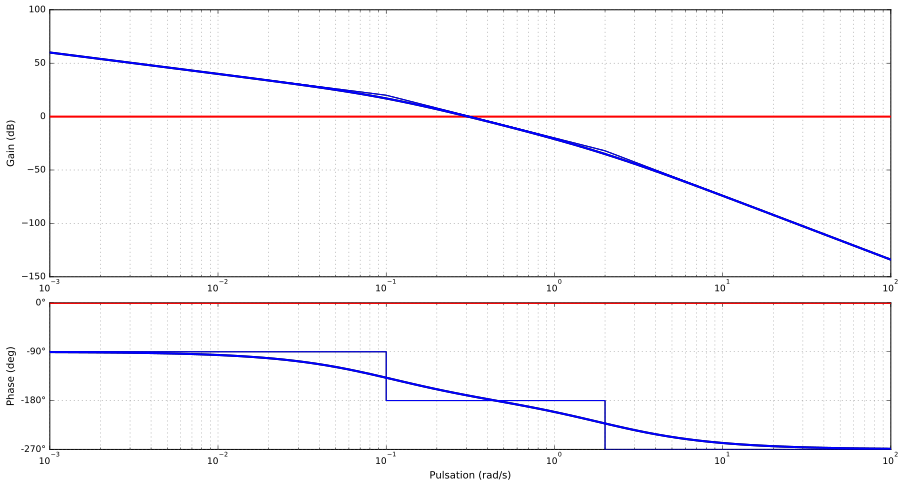
\includegraphics[width=\linewidth]{fig_03}
%\end{center}
%\end{minipage}\hfill
%\begin{minipage}[c]{.46\linewidth}
%\begin{center}
%\includegraphics[width=.9\linewidth]{fig_01}
%\end{center}
%\end{minipage}

\ifprof
\else
\fi

%
%\begin{center}
%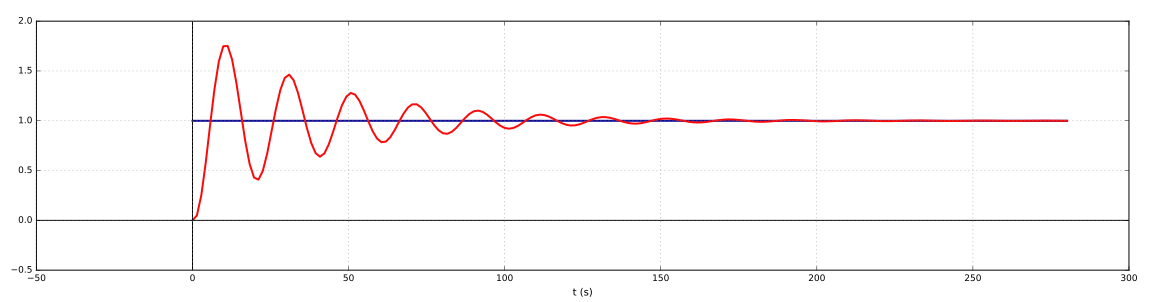
\includegraphics[width=\linewidth]{fig_02}
%\end{center}
%
%\begin{center}
%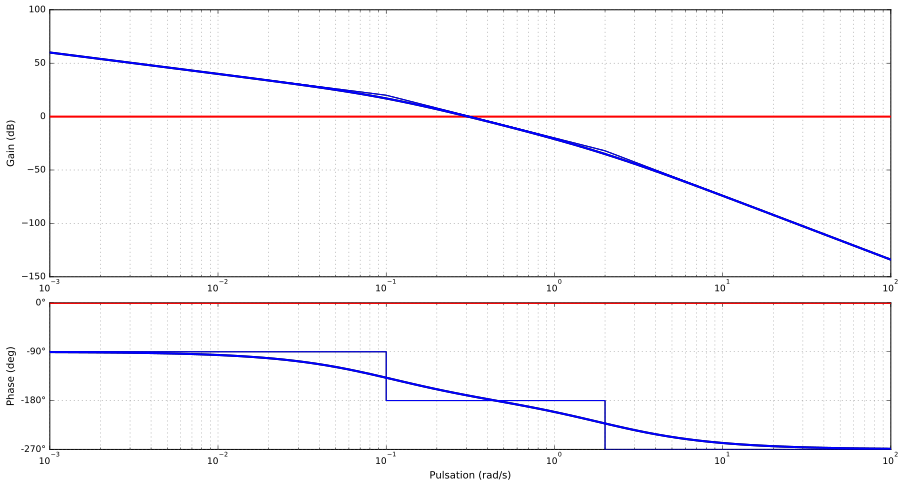
\includegraphics[width=\linewidth]{fig_03}
%\end{center}
%
%\begin{center}
%\includegraphics[width=.8\linewidth]{fig_04}
%\end{center}



%\end{document}
%
%\subsection*{Exercice 3 -- Applications du critère du Revers}
%
%\subparagraph*{}\textit{On donne ci-dessous les lieux de transferts de plusieurs FTBO. Déterminer, à l'aide du critère du Revers si les systèmes sont stables en BF.}
%\subparagraph*{}\textit{Pour les systèmes stables déterminer les marges de gain et de phase.}
%
%\end{multicols}
%
%\begin{center}
%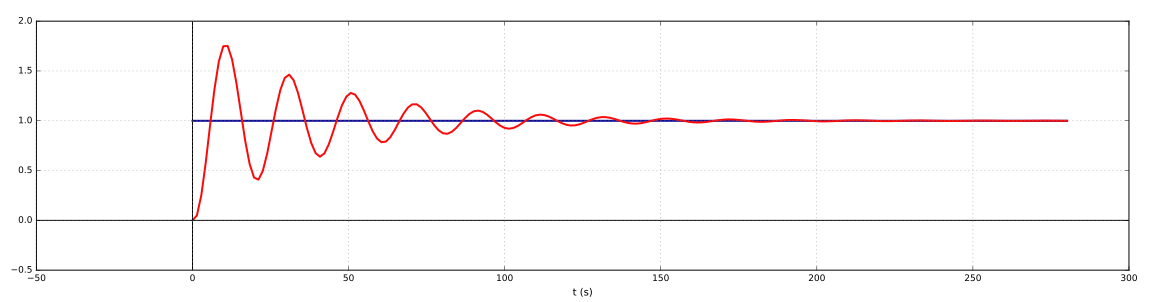
\includegraphics[width=\linewidth]{fig_02}
%\end{center}
%
%\begin{center}
%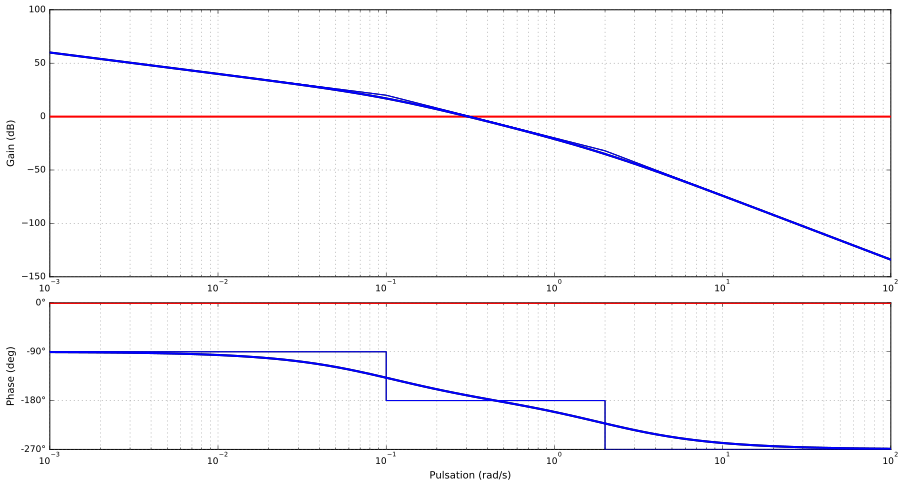
\includegraphics[width=\linewidth]{fig_03}
%\end{center}
%
%\begin{center}
%\includegraphics[width=.8\linewidth]{fig_04}
%\end{center}
%


